% ======================================================================
% MetaFlow Paper Deep-Dive: Interview Presentation Slides
% Candidate: Partha Pratim Saha | GreenFieldData PhD-L
% Purpose: Demonstrate understanding of MetaFlow for PhD interview
%          Reference paper: Tagliabue et al. (2023) -- MLSys
%          Reference book:  Tuulos (2022) -- Manning
% ======================================================================
\documentclass[10pt,aspectratio=169]{beamer}

\usetheme{Madrid}
\usecolortheme{seahorse}
\usepackage{tikz}
\usetikzlibrary{arrows.meta,positioning,shapes.geometric}
\usepackage{listings}
\usepackage{booktabs}
\usepackage{xcolor}
\usepackage{amsmath}
\usepackage[T1]{fontenc}

\definecolor{mfblue}{RGB}{0,60,110}
\definecolor{mfgreen}{RGB}{34,120,34}
\definecolor{mforange}{RGB}{200,90,20}
\definecolor{mfgray}{RGB}{90,90,90}
\definecolor{codebg}{RGB}{250,250,248}

\setbeamercolor{frametitle}{bg=mfblue,fg=white}
\setbeamercolor{structure}{fg=mfblue}
\setbeamercolor{block title}{bg=mfblue!80,fg=white}
\setbeamercolor{alerted text}{fg=mforange}
\setbeamerfont{frametitle}{size=\normalsize,series=\bfseries}
\setbeamerfont{block title}{size=\small,series=\bfseries}

\lstset{
  basicstyle=\tiny\ttfamily,
  keywordstyle=\color{mfblue}\bfseries,
  commentstyle=\color{mfgreen!70!black},
  stringstyle=\color{mforange},
  backgroundcolor=\color{codebg},
  frame=single,framerule=0.3pt,
  language=Python,
  breaklines=true,
  showstringspaces=false,
  numbers=left,numberstyle=\tiny\color{mfgray},
  xleftmargin=1.2em,
}

\title[MetaFlow: Interview Deep-Dive]{MetaFlow as Scientific Infrastructure for Agricultural AI}
\subtitle{A PhD Interview Perspective on Tagliabue et al.\ (2023) and Tuulos (2022)}
\author{Partha Pratim Saha}
\institute{GreenFieldData MSCA PhD-L\\UCBLyon1 / UniMI}
\date{Interview, May 2026}

% ---- Helper commands -----------------------------------------------
\newcommand{\V}[1]{\textcolor{mforange}{\textbf{V#1}}}
\newcommand{\Key}[1]{\textcolor{mfblue}{\textbf{#1}}}

\begin{document}

% ====================================================================
% SLIDE 1: Title
% ====================================================================
\begin{frame}
\titlepage
\vspace{-0.3cm}
\begin{center}
\small
\textbf{Two sources I will discuss today:}\\
\begin{tabular}{ll}
Paper: & Tagliabue, Tuulos et al., \emph{You Do Not Need a Bigger Boat} (MLSys 2023)\\
Book:  & Tuulos, \emph{Effective Data Science Infrastructure} (Manning, 2022)\\
\end{tabular}
\end{center}
\end{frame}

% ====================================================================
% SLIDE 2: The Core Problem MetaFlow Solves
% ====================================================================
\begin{frame}{The Problem: The Dev-to-Production Gap in ML}

\begin{columns}
\begin{column}{0.5\textwidth}
\begin{block}{Classic ML Project Failure Pattern}
\begin{enumerate}\small
  \item Notebook prototype works \checkmark
  \item Rewrite for production: 6 months
  \item Rewrite loses reproducibility
  \item New batch: start over
  \item \alert{Never shipped, or shipped wrongly}
\end{enumerate}
\end{block}
\vspace{0.3cm}
\begin{alertblock}{Root Cause (Tagliabue et al.)}
\small ``The main cost is not compute --- it is \textbf{abstraction mismatch}
between data scientists and infrastructure engineers.''
\end{alertblock}
\end{column}
\begin{column}{0.5\textwidth}
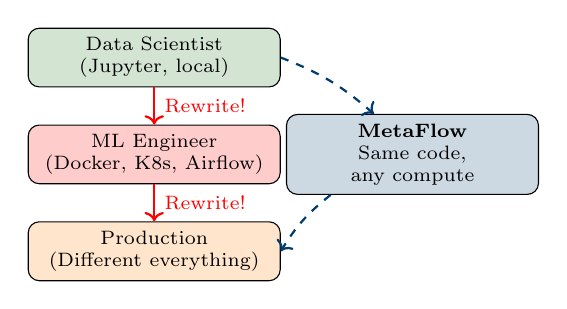
\begin{tikzpicture}[scale=0.82, every node/.style={font=\scriptsize}]
  \node[draw,rounded corners,fill=mfgreen!20,minimum width=3.2cm,minimum height=0.7cm,align=center] (ds) at (0,3) {Data Scientist\\(Jupyter, local)};
  \node[draw,rounded corners,fill=red!20,minimum width=3.2cm,minimum height=0.7cm,align=center] (eng) at (0,1.5) {ML Engineer\\(Docker, K8s, Airflow)};
  \node[draw,rounded corners,fill=orange!20,minimum width=3.2cm,minimum height=0.7cm,align=center] (prod) at (0,0) {Production\\(Different everything)};
  \draw[->,thick,red] (ds) -- node[right]{\alert{Rewrite!}} (eng);
  \draw[->,thick,red] (eng) -- node[right]{\alert{Rewrite!}} (prod);
  \node[draw,rounded corners,fill=mfblue!20,minimum width=3.2cm,minimum height=0.7cm,align=center] (mf) at (4,1.5) {\textbf{MetaFlow}\\Same code,\\any compute};
  \draw[->,thick,mfblue,dashed] (ds.east) to[bend left=10] (mf);
  \draw[->,thick,mfblue,dashed] (mf) to[bend right=10] (prod.east);
\end{tikzpicture}
\end{column}
\end{columns}

\vspace{0.2cm}
\Key{MetaFlow's answer:} Prototype and production are \emph{the same code}. The abstraction continuity is not a convenience --- it is the scientific contribution.

\end{frame}

% ====================================================================
% SLIDE 3: MetaFlow Philosophy -- Abstraction Continuity
% ====================================================================
\begin{frame}{MetaFlow Philosophy: Abstraction Continuity as a Research Principle}

\begin{block}{Core Insight (Tuulos, 2022, p.\ 3)}
\small ``A data scientist should be able to write code that runs on their laptop
and on a cloud cluster without changing a single line of business logic.
Infrastructure is a \emph{decorator}, not a rewrite.''
\end{block}

\begin{columns}
\begin{column}{0.55\textwidth}
\small
\textbf{What MetaFlow provides:}
\begin{itemize}
  \item \Key{DAG execution}: steps are Python methods, graph is declared via \texttt{self.next()}
  \item \Key{Artifact versioning}: every step output is a versioned artifact with run ID
  \item \Key{Compute decorators}: \texttt{@batch}, \texttt{@kubernetes}, \texttt{@conda}, \texttt{@resources} --- same code, different compute
  \item \Key{Run lineage}: inspect any historical run, any step, any artifact
  \item \Key{Resume}: restart from any step after failure
\end{itemize}

\vspace{0.2cm}
\textbf{What it deliberately does \emph{not} do:}
\begin{itemize}
  \item Replace data stores (use S3, Postgres, etc.)
  \item Schedule (use cron or Airflow for that)
  \item Replace model registries (MLflow, W\&B)
\end{itemize}
\end{column}
\begin{column}{0.42\textwidth}
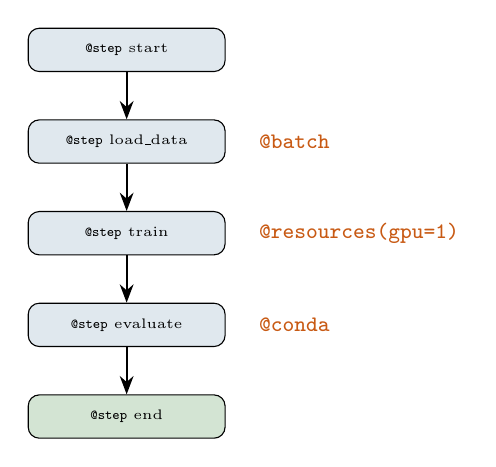
\begin{tikzpicture}[scale=0.75, node distance=0.6cm, >=Stealth, every node/.style={font=\tiny}]
  \node[draw,rounded corners,fill=mfblue!12,minimum width=2.5cm,minimum height=0.55cm,align=center] (s) {\texttt{@step} start};
  \node[draw,rounded corners,fill=mfblue!12,minimum width=2.5cm,minimum height=0.55cm,align=center,below=of s] (a) {\texttt{@step} load\_data};
  \node[draw,rounded corners,fill=mfblue!12,minimum width=2.5cm,minimum height=0.55cm,align=center,below=of a] (b) {\texttt{@step} train};
  \node[draw,rounded corners,fill=mfblue!12,minimum width=2.5cm,minimum height=0.55cm,align=center,below=of b] (c) {\texttt{@step} evaluate};
  \node[draw,rounded corners,fill=mfgreen!20,minimum width=2.5cm,minimum height=0.55cm,align=center,below=of c] (e) {\texttt{@step} end};
  \draw[->,thick] (s)--(a); \draw[->,thick] (a)--(b);
  \draw[->,thick] (b)--(c); \draw[->,thick] (c)--(e);
  \node[right=0.3cm of a, color=mforange] {\footnotesize \texttt{@batch}};
  \node[right=0.3cm of b, color=mforange] {\footnotesize \texttt{@resources(gpu=1)}};
  \node[right=0.3cm of c, color=mforange] {\footnotesize \texttt{@conda}};
\end{tikzpicture}
\end{column}
\end{columns}

\end{frame}

% ====================================================================
% SLIDE 4: The Three Vs -- Velocity
% ====================================================================
\begin{frame}[fragile]{V1 --- Velocity: Iteration Without Infrastructure Overhead}

\begin{block}{Problem (Tagliabue et al., 2023)}
\small In ML research, the cost of changing one step should not force re-running all steps.
In agricultural AI: re-ingesting 3 years of sensor data just to test a new calibration method
wastes research time.
\end{block}

\begin{columns}
\begin{column}{0.52\textwidth}
\begin{lstlisting}[title={\scriptsize Iterating on calibration step only}]
# Run full pipeline first time:
python agritalk_flow.py run

# Saved artifact: run/1234/calibrate/data

# Iterate on calibration ONLY -- no re-ingestion:
python agritalk_flow.py run \
  --start-step calibrate

# MetaFlow reuses all upstream artifacts.
# Supervisor in Lyon can inspect:
from metaflow import Run
r = Run("AgriTalkFlow/1234")
print(r["calibrate"].task.data.ece_score)
\end{lstlisting}
\end{column}
\begin{column}{0.45\textwidth}
\small
\textbf{Why this matters for PhD research:}
\begin{itemize}
  \item Year 1: iterate on conformal calibration (C1) without re-ingesting sensor corpus
  \item Year 2: iterate on BVF attribution (C2) without re-running fine-tuning
  \item Year 3: iterate on federated evaluation without re-training per farm
\end{itemize}

\vspace{0.3cm}
\begin{alertblock}{Key point for interview}
\small \textbf{Velocity is not about running faster.} It is about isolating the research variable you are actually changing. MetaFlow enforces this by design.
\end{alertblock}
\end{column}
\end{columns}

\end{frame}

% ====================================================================
% SLIDE 5: The Three Vs -- Validation
% ====================================================================
\begin{frame}[fragile]{V2 --- Validation: Artifact-Level Inspection Across Sites}

\begin{block}{Problem in Joint PhD Context}
\small How does a supervisor in Lyon verify that the model I trained
and evaluated in Milan used the \emph{correct calibration set}?
With a Git repo, they can check code. With MetaFlow, they can inspect the \emph{exact artifact} used at every step.
\end{block}

\begin{columns}
\begin{column}{0.54\textwidth}
\begin{lstlisting}[title={\scriptsize Cross-site validation (Lyon + Milan)}]
from metaflow import Run, namespace

# Supervisor in Lyon checks Milan run:
namespace("partha@unimi")
run = Run("AgriTalkFlow/5678")

# Inspect the exact calibration set:
cal_set = run["calibrate"].task.data.cal_set
print(f"Calibration size: {len(cal_set)}")
print(f"Coverage achieved: "
      f"{run['calibrate'].task.data.coverage}")

# Inspect model artifact:
model = run["finetune"].task.data.model_path
print(f"Model: {model}")
print(f"Git SHA: "
      f"{run.data.git_sha}")  # automatic
\end{lstlisting}
\end{column}
\begin{column}{0.43\textwidth}
\small
\textbf{What this enables:}
\begin{itemize}
  \item Dr.\ Vargas-Solar (Lyon) can validate C1 calibration artifacts remotely
  \item Prof.\ Oberti (Milan) can validate C2 attribution runs without GPU access
  \item Cross-institution paper co-authorship is backed by \emph{verifiable shared artifact state}
  \item Version mismatches are impossible: artifact ID encodes exact environment
\end{itemize}
\vspace{0.2cm}
\textbf{Contrast with Jupyter notebooks:}\\
``It worked on my machine'' is a paper validity crisis, not just an inconvenience.
\end{column}
\end{columns}

\end{frame}

% ====================================================================
% SLIDE 6: The Three Vs -- Versioning
% ====================================================================
\begin{frame}[fragile]{V3 --- Versioning: Complete Scientific Run Lineage}

\begin{block}{What MetaFlow Versions (Tuulos, 2022, Ch.\ 4)}
\small Every run receives an immutable run ID. Every artifact (model weights, datasets, evaluation
metrics, calibration sets) is content-addressed and retained indefinitely.
\end{block}

\begin{columns}
\begin{column}{0.54\textwidth}
\begin{lstlisting}[title={\scriptsize Seasonal regression detection}]
from metaflow import Flow
import pandas as pd

flow = Flow("AgriTalkFinetuneFlow")

# Compare all runs across seasons:
records = []
for run in flow.runs():
    if run.successful:
        records.append({
            "run_id": run.id,
            "season": run.data.season_tag,
            "ece": run.data.ece_score,
            "macro_f1": run.data.macro_f1,
            "git_sha": run.data.git_sha,
        })

df = pd.DataFrame(records)
# Detect calibration drift:
drift = df.groupby("season")["ece"].mean()
print(drift)  # Plots seasonal ECE trend
\end{lstlisting}
\end{column}
\begin{column}{0.43\textwidth}
\small
\textbf{PhD-level value of versioning:}
\begin{itemize}
  \item Seasonal replay: \emph{``Would Year~1 calibration have worked on Year~2 data?''} --- answerable with evidence
  \item Model regression detection across research iterations
  \item Complete provenance chain: corpus $\to$ fine-tune $\to$ calibrate $\to$ evaluate $\to$ paper metric
  \item Every number in every paper can be traced back to an exact run artifact
\end{itemize}

\vspace{0.2cm}
\begin{alertblock}{Interviewer note}
\small This is why MetaFlow is a \emph{scientific necessity} for C4, not just a convenient tool.
\end{alertblock}
\end{column}
\end{columns}

\end{frame}

% ====================================================================
% SLIDE 7: @step Functions and Decorator Semantics
% ====================================================================
\begin{frame}[fragile]{Step Functions and Decorator Semantics}

\begin{columns}
\begin{column}{0.58\textwidth}
\begin{lstlisting}[title={\scriptsize Decorator semantics: same code, different compute}]
from metaflow import FlowSpec, step, batch, conda

class AgriTalkFlow(FlowSpec):

    @step
    def start(self):
        """Run locally (lightweight init)"""
        self.season = "lyon_spring_2027"
        self.next(self.load_sensor_data)

    @conda(libraries={"kafka-python": "2.0.2"})
    @step
    def load_sensor_data(self):
        """Load from Kafka -- reproducible snapshot"""
        # Reads from archived Kafka snapshot
        self.sensor_df = load_kafka_snapshot(
            topic="agritalk.sensor.raw",
            timestamp=self.season_start_ts
        )
        self.next(self.calibrate)

    @batch(cpu=8, memory=16000)  # Cloud GPU
    @step
    def calibrate(self):
        """Conformal calibration -- runs on AWS Batch"""
        from calibration import conformal_fit
        self.cal_set, self.coverage = \
            conformal_fit(self.sensor_df, alpha=0.05)
        self.next(self.end)

    @step
    def end(self):
        print(f"Coverage: {self.coverage:.3f}")
\end{lstlisting}
\end{column}
\begin{column}{0.39\textwidth}
\small
\textbf{Key decorator behaviors:}
\begin{itemize}
  \item \texttt{@step}: marks a DAG node; output is automatically persisted as artifact
  \item \texttt{@batch}: executes on AWS Batch; same code, no rewrite
  \item \texttt{@conda}: pins exact dependency versions; reproducibility across machines
  \item \texttt{@kubernetes}: runs on Kubernetes pod (UCBLyon1 cluster)
  \item \texttt{@resources}: specifies CPU/GPU/memory per step
  \item \texttt{@retry}: automatic failure recovery
  \item \texttt{@timeout}: step-level safety timeout
\end{itemize}

\vspace{0.3cm}
\Key{Key insight:} \texttt{self.sensor\_df} is automatically saved --- no \texttt{pickle}, no \texttt{joblib}, no manual artifact management.
\end{column}
\end{columns}

\end{frame}

% ====================================================================
% SLIDE 8: DAG as Scientific Object
% ====================================================================
\begin{frame}{DAG as Scientific Object (Not Just a Workflow Tool)}

\begin{columns}
\begin{column}{0.5\textwidth}
\small
\textbf{Tagliabue et al.\ (2023) key argument:}\\
The DAG is not a deployment artifact --- it \emph{is} the scientific hypothesis.

\vspace{0.3cm}
\textbf{In classical ML:}\\
``My experiment'' = a notebook + ad-hoc results

\vspace{0.3cm}
\textbf{In MetaFlow:}\\
``My experiment'' = a DAG with versioned artifacts at every step = reproducible scientific object

\vspace{0.3cm}
\begin{block}{DAG Card $\equiv$ Model Card (Tagliabue et al.)}
\small The DAG Card (analogous to Model Card) documents: inputs, outputs, each step's purpose, provenance, compute requirements, and test criteria --- at the \emph{pipeline} level, not just the model level.
\end{block}
\end{column}
\begin{column}{0.46\textwidth}
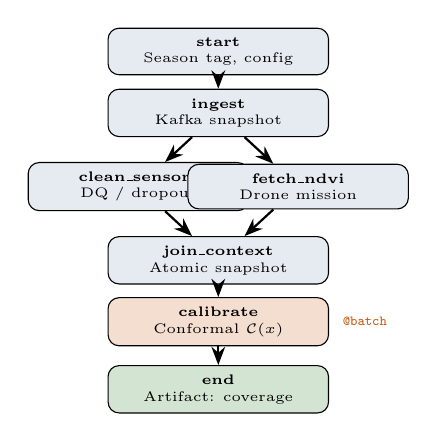
\begin{tikzpicture}[scale=0.78, >=Stealth, every node/.style={font=\tiny}]
  \node[draw,rounded corners,fill=mfblue!10,minimum width=2.8cm,minimum height=0.55cm,align=center] (a) at (0,5.5) {\textbf{start}\\Season tag, config};
  \node[draw,rounded corners,fill=mfblue!10,minimum width=2.8cm,minimum height=0.55cm,align=center] (b) at (0,4.5) {\textbf{ingest}\\Kafka snapshot};
  \node[draw,rounded corners,fill=mfblue!10,minimum width=2.8cm,minimum height=0.55cm,align=center] (c) at (-1.3,3.3) {\textbf{clean\_sensors}\\DQ / dropout};
  \node[draw,rounded corners,fill=mfblue!10,minimum width=2.8cm,minimum height=0.55cm,align=center] (d) at (1.3,3.3) {\textbf{fetch\_ndvi}\\Drone mission};
  \node[draw,rounded corners,fill=mfblue!10,minimum width=2.8cm,minimum height=0.55cm,align=center] (e) at (0,2.1) {\textbf{join\_context}\\Atomic snapshot};
  \node[draw,rounded corners,fill=mforange!20,minimum width=2.8cm,minimum height=0.55cm,align=center] (f) at (0,1.1) {\textbf{calibrate}\\Conformal $\mathcal{C}(x)$};
  \node[draw,rounded corners,fill=mfgreen!20,minimum width=2.8cm,minimum height=0.55cm,align=center] (g) at (0,0) {\textbf{end}\\Artifact: coverage};
  \draw[->,thick] (a)--(b); \draw[->,thick] (b)--(c); \draw[->,thick] (b)--(d);
  \draw[->,thick] (c)--(e); \draw[->,thick] (d)--(e);
  \draw[->,thick] (e)--(f); \draw[->,thick] (f)--(g);
  \node[right=0.05cm of f,color=mforange]{\texttt{@batch}};
\end{tikzpicture}
\end{column}
\end{columns}

\end{frame}

% ====================================================================
% SLIDE 9: Why MetaFlow is Scientifically Necessary for Agricultural AI
% ====================================================================
\begin{frame}{Why MetaFlow is Scientifically Necessary for This PhD}

\begin{alertblock}{The Non-Stationarity Problem (unique to agricultural AI)}
\small An agricultural AI experiment is not stationary: weather, crop lifecycle, weed pressure, soil variation, pest resistance, and operator vocabulary differ across seasons, farms, and years. A model trained in Lyon spring is evaluated against Milan autumn. \textbf{Without explicit versioning of environmental state, comparison is scientifically invalid.}
\end{alertblock}

\vspace{0.3cm}
\begin{columns}
\begin{column}{0.33\textwidth}
\begin{block}{\V{elocity} in Agriculture}
\small Re-calibrate conformal prediction (C1) for spring wheat without re-ingesting 18 months of sensor data.
\end{block}
\end{column}
\begin{column}{0.33\textwidth}
\begin{block}{\V{alidation} in Agriculture}
\small Dr.\ Vargas-Solar verifies a BVF attribution run (C2) in Lyon using the exact artifact from Milan --- not a copy, the same artifact.
\end{block}
\end{column}
\begin{column}{0.33\textwidth}
\begin{block}{\V{ersioning} in Agriculture}
\small \emph{``Was Year~1 calibration still valid in Year~3?''} Seasonal replay answers this with evidence, not assumption.
\end{block}
\end{column}
\end{columns}

\vspace{0.4cm}
\begin{center}
\small\textbf{MetaFlow is contribution C4 --- infrastructure that makes C1, C2, C3 reproducibly publishable.}\\
Not a research question; a scientific validity guarantee.
\end{center}

\end{frame}

% ====================================================================
% SLIDE 10: Non-Stationarity and Seasonal Replay
% ====================================================================
\begin{frame}[fragile]{Seasonal Replay: A PhD-Level MetaFlow Feature}

\begin{block}{Core Question This Enables}
\small \emph{``Would the HITL policy calibrated on Lyon winter 2027 data have correctly triggered during UniMI spring 2028 early-season spraying?''}\\
Without MetaFlow: answered with guesswork or a new experiment. With MetaFlow: answered by replaying the archived calibration step against archived sensor snapshots.
\end{block}

\begin{columns}
\begin{column}{0.56\textwidth}
\begin{lstlisting}[title={\scriptsize Seasonal replay implementation}]
from metaflow import Run

# Load Lyon winter 2027 calibration artifacts:
winter_run = Run("AgriTalkFlow/1234")
cal_set_winter = winter_run.data.cal_set
alpha_winter = winter_run.data.alpha

# Load Milan spring 2028 sensor snapshot:
spring_run = Run("AgriTalkFlow/5678")
sensor_spring = spring_run.data.sensor_df

# Replay calibration against new season:
from calibration import conformal_eval
coverage_spring = conformal_eval(
    cal_set=cal_set_winter,
    test_data=sensor_spring,
    alpha=alpha_winter
)

print(f"Cross-season coverage: {coverage_spring:.3f}")
# If < 0.95: seasonal recalibration is needed.
# This is an empirical finding, not an assumption.
\end{lstlisting}
\end{column}
\begin{column}{0.41\textwidth}
\small
\textbf{Scientific value:}
\begin{itemize}
  \item Tests whether conformal exchangeability assumption holds across seasons (RQ1 body)
  \item Provides calibration drift evidence to justify adaptive recalibration mechanism
  \item Every replay is a traceable experiment with its own run ID
  \item Requires \emph{zero additional data collection} --- uses archived artifacts
\end{itemize}

\vspace{0.3cm}
\textbf{Without versioning:}
``I believe the calibration would have transferred'' (not publishable)

\textbf{With versioning:}
``The measured cross-season coverage was 0.91 vs.\ the nominal 0.95 target, triggering adaptive recalibration'' (publishable)
\end{column}
\end{columns}

\end{frame}

% ====================================================================
% SLIDE 11: MetaFlow vs. Alternatives
% ====================================================================
\begin{frame}{MetaFlow vs.\ Alternatives: Principled Comparison}

\begin{center}\small
\begin{tabular}{@{}lccccl@{}}
\toprule
\textbf{Tool} & \textbf{Prototype$\to$Prod} & \textbf{Artifact V.} & \textbf{Resume} & \textbf{Compute Decorator} & \textbf{PhD fit} \\
\midrule
\textbf{MetaFlow}   & \textcolor{mfgreen}{$\checkmark$} Same code & \textcolor{mfgreen}{$\checkmark$} Full & \textcolor{mfgreen}{$\checkmark$} Any step & \textcolor{mfgreen}{$\checkmark$} @batch/@k8s & Excellent \\
Airflow    & \textcolor{red}{$\times$} DAG = deployment & \textcolor{red}{$\times$} None & \textcolor{mforange}{$\sim$} DAG-level & Plugin only & Scheduling only \\
Kubeflow   & \textcolor{red}{$\times$} K8s rewrite & \textcolor{mforange}{$\sim$} Limited & \textcolor{mforange}{$\sim$} Limited & \textcolor{mfgreen}{$\checkmark$} Native K8s & Overkill \\
MLflow     & \textcolor{red}{$\times$} Experiment only & \textcolor{mforange}{$\sim$} Model-level & \textcolor{red}{$\times$} None & \textcolor{red}{$\times$} None & No orchestration \\
W\&B       & \textcolor{red}{$\times$} Logging only & \textcolor{mforange}{$\sim$} Run-level & \textcolor{red}{$\times$} None & \textcolor{red}{$\times$} None & No pipelines \\
\bottomrule
\end{tabular}
\end{center}

\vspace{0.2cm}
\begin{columns}
\begin{column}{0.48\textwidth}
\begin{block}{Why not Airflow?}
\small Airflow schedules computational tasks but does not provide artifact versioning, prototype continuity, or step-level artifact inspection. My research requires all three.
\end{block}
\end{column}
\begin{column}{0.48\textwidth}
\begin{block}{Why not Kubeflow?}
\small Kubeflow provides Kubernetes-native ML pipelines but requires infrastructure expertise beyond a PhD scope. MetaFlow's \texttt{@kubernetes} decorator provides the same compute access with prototype continuity.
\end{block}
\end{column}
\end{columns}

\end{frame}

% ====================================================================
% SLIDE 12: Code Walkthrough -- AgriTalkFlow
% ====================================================================
\begin{frame}[fragile]{Code Walkthrough: AgriTalkFlow in 12 Steps}

\begin{columns}
\begin{column}{0.56\textwidth}
\begin{lstlisting}[title={\scriptsize agritalk\_flow.py -- simplified structure}]
from metaflow import FlowSpec, step, Parameter
from metaflow import batch, conda, resources

class AgriTalkFlow(FlowSpec):

    season = Parameter("season",
                       default="lyon_spring_2027")
    alpha  = Parameter("alpha",
                       default=0.05, type=float)

    @step
    def start(self): self.next(self.ingest)

    @conda(libraries={"kafka-python":"2.0.2"})
    @step
    def ingest(self):
        self.sensor_df = load_kafka(self.season)
        self.next(self.clean, self.fetch_ndvi)

    @step
    def clean(self):
        self.clean_df = dq_check(self.sensor_df)
        self.next(self.join_context)

    @step
    def fetch_ndvi(self):
        self.ndvi = load_ndvi(self.season)
        self.next(self.join_context)

    @step
    def join_context(self, inputs):
        self.context = merge(inputs.clean.clean_df,
                             inputs.fetch_ndvi.ndvi)
        self.next(self.calibrate)

    @batch(cpu=4, memory=8000)
    @step
    def calibrate(self):
        self.cal_set, self.coverage = \
            conformal_fit(self.context, self.alpha)
        self.next(self.evaluate)

    @step
    def evaluate(self):
        self.metrics = eval_on_agroNLP(self.cal_set)
        self.next(self.end)

    @step
    def end(self): pass
\end{lstlisting}
\end{column}
\begin{column}{0.41\textwidth}
\small
\textbf{Pipeline patterns shown:}
\begin{itemize}
  \item \Key{Fan-out}: \texttt{ingest $\to$ clean + fetch\_ndvi} (parallel)
  \item \Key{Fan-in}: \texttt{join\_context(inputs)} merges fan-out results
  \item \Key{Parameters}: season and alpha passed from CLI, tracked per run
  \item \Key{@conda}: pins dependencies per step
  \item \Key{@batch}: cloud execution for calibration
\end{itemize}

\vspace{0.3cm}
\textbf{Running:}
\begin{lstlisting}[language=bash,frame=none,numbers=none]
# Local prototype:
python agritalk_flow.py run

# With different season:
python agritalk_flow.py run \
  --season milan_autumn_2028

# Resume from calibrate:
python agritalk_flow.py run \
  --start-step calibrate
\end{lstlisting}
\end{column}
\end{columns}

\end{frame}

% ====================================================================
% SLIDE 13: Anticipated Questions from Interview Committee
% ====================================================================
\begin{frame}{Anticipated Interview Questions and My Answers}

\begin{block}{Q1: Why not just use Jupyter notebooks with Git?}
\small Git versions \emph{code}; MetaFlow versions \emph{artifacts}. Running the same notebook twice with different random seeds or different upstream data produces different results that Git cannot distinguish. MetaFlow's run IDs provide this artifact identity. In a 3-year multi-site PhD, code versioning without artifact versioning is insufficient.
\end{block}

\begin{block}{Q2: Is MetaFlow mature enough for research, not just production?}
\small Tagliabue et al.\ (2023) demonstrate exactly this: researchers at Coveo used MetaFlow to publish reproducible ML papers. The fact that MetaFlow originated at Netflix (Tuulos, 2022) is evidence of production maturity; its adoption in research contexts is the contribution of the paper I am referencing.
\end{block}

\begin{block}{Q3: Could you switch to Airflow if MetaFlow were unavailable?}
\small Airflow would handle scheduling and task orchestration, but I would lose step-level artifact versioning and the prototype-to-production continuity. I would likely add MLflow for experiment tracking on top. This is why MetaFlow is the right architectural choice rather than an arbitrary one.
\end{block}

\end{frame}

% ====================================================================
% SLIDE 14: My PhD Research Plan via MetaFlow
% ====================================================================
\begin{frame}{How MetaFlow Structures My 3-Year Research Plan}

\begin{center}\small
\begin{tabular}{@{}clll@{}}
\toprule
\textbf{Year} & \textbf{MetaFlow Pipeline} & \textbf{Key Steps} & \textbf{Seasonal Replay Use} \\
\midrule
1 & \texttt{AgriTalkIngestFlow} & ingest $\to$ clean $\to$ register & Baseline: Lyon spring 2027 \\
1 & \texttt{AgriTalkFinetuneFlow} & fine-tune $\to$ eval $\to$ calibrate (C1) & Calibration artifact archived \\
\midrule
2 & \texttt{AgriTalkStreamFlow} & Kafka $\to$ context $\to$ TSGA (C3) & Lyon artifacts replayed at Milan \\
2 & \texttt{AgriTalkBVFFlow} & attribution $\to$ verifier (C2) & Cross-season BVF stability \\
\midrule
3 & \texttt{AgriTalkFederatedFlow} & per-farm $\to$ aggregate $\to$ eval & All seasons, all farms \\
3 & \texttt{AgriTalkHITLStudyFlow} & user study data $\to$ trust calibration & Replay for counter-factual \\
\bottomrule
\end{tabular}
\end{center}

\vspace{0.3cm}
\begin{columns}
\begin{column}{0.6\textwidth}
\small
\textbf{Every paper submission includes:}
\begin{itemize}
  \item Run ID(s) for all reported numbers
  \item Artifact hash for model weights, calibration sets, evaluation metrics
  \item Seasonal tag: which farm, which season, which sensor configuration
  \item Reproducibility checklist via DAG Card (Tagliabue et al., 2021)
\end{itemize}
\end{column}
\begin{column}{0.37\textwidth}
\begin{alertblock}{Research integrity note}
\small Artifact versioning is not optional in agricultural AI. Seasonal variation means ``I ran the same code'' is insufficient: the data and environment also varied.
\end{alertblock}
\end{column}
\end{columns}

\end{frame}

% ====================================================================
% SLIDE 15: Questions for Supervisors
% ====================================================================
\begin{frame}{Questions I Would Ask My Supervisors About MetaFlow}

\begin{block}{For Dr.\ Vargas-Solar (Lyon / Distributed Data)}
\begin{enumerate}\small
  \item How are sensor data snapshots currently archived at UCBLyon1? Is there a standard schema or naming convention I should build the Kafka-to-Metaflow adapter against?
  \item Is there institutional GPU access (or AWS budget) for \texttt{@batch} steps, or should I architect C1 calibration to run on CPU-only clusters for Year 1?
  \item Are there existing ProBayes pipelines I should ensure MetaFlow integrates with cleanly (artifact format, schema agreements)?
\end{enumerate}
\end{block}

\begin{block}{For Prof.\ Oberti (Milan / Robotics / Agriculture)}
\begin{enumerate}\small
  \item Which sensors are instrumented on the UniMI experimental farm? Which topics would you recommend as ground-truth sources for NDVI and spray event logging?
  \item Is there an existing software interface between the farm robots and ROS2 that I should treat as fixed, or is there flexibility in the command interface design for the AgriTalk HITL gate?
  \item For the Year 2 operator study, how many operators and agronomists can I realistically recruit for the HITL trust calibration experiment?
\end{enumerate}
\end{block}

\vspace{0.2cm}
\begin{center}
\small\textit{Thank you. I welcome any questions about the technical or research framing above.}
\end{center}

\end{frame}

\end{document}
